\section{Branch and Bound} \label{sec:branch-and-bound}

Branch and Bound é uma técnica para algoritmos que visa melhorar
o tempo de processamento ao eliminar as soluções-candidato que claramente
não se aplicam e/ou não ajudam a resolver o problema. Esse método geralmente
é aplicado em problemas que têm soluções finitas, no qual as soluções podem 
ser representadas como uma sequência de opções. 

A primeira parte da técnica Branch and Bound pede que o algoritmo trate
as possíveis soluções como se estivessem em uma estrutura de árvore, onde 
os nós da árvore são utilizados como partes de possíveis soluções garante 
que todas soluções sejam consideradas.

\subsection{Problema da Mochila}

\begin{figure}[ht]
    \centering
    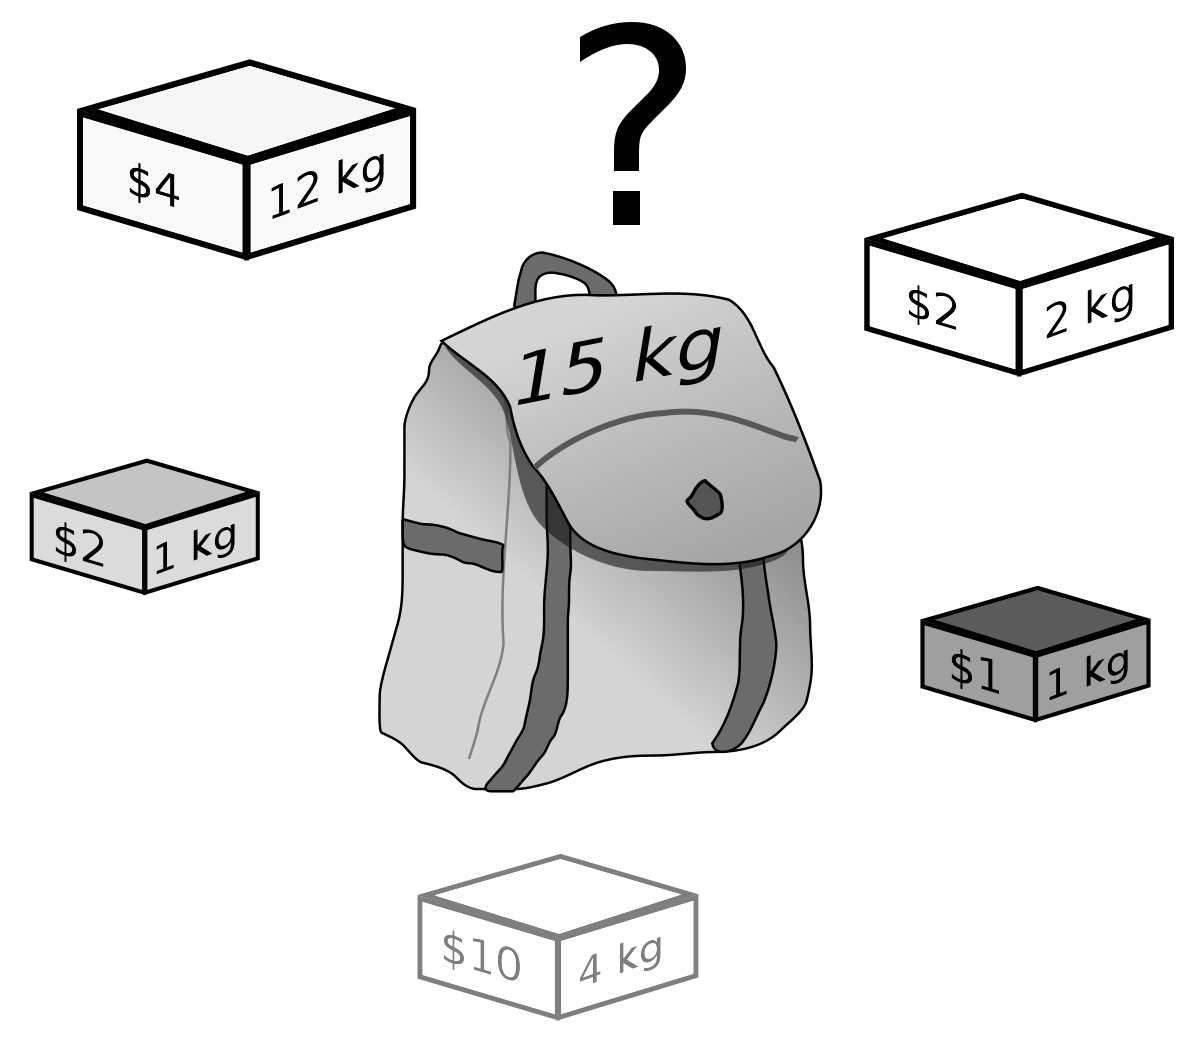
\includegraphics[width=.5\textwidth]{knapsack.png}
    \caption{Ilustração do problema da mochila}
    \label{fig:knapsack}
\end{figure}


O problema escolhido para mostrar essa estratégia é o problema do 0/1 Knapsack.
A ideia por trás dele é um ladrão que quer roubar uma casa, mas sua mochila so 
aguenta carregar um peso P1. Existem vários items na casa, cada um com seu valor V e peso P2. Escolha os items específicos que vão maximizar o valor roubado pelo ladrão de forma que a soma dos pesos dos items nunca seja maior que P1.

Podemos ilustrar as combinações de items em uma estrutura de árvore, de forma 
que cada nó é um item que o ladrão pode roubar, e um caminho percorrendo N nós 
significa um conjunto de N items.

\begin{figure}[ht]
    \centering
    \begin{forest}
      for tree={
          grow=south,
          circle, draw, minimum size=3ex, inner sep=5pt,
          s sep=15mm
              }
      [1
          [2, edge label={node[midway,above left,font=\scriptsize]{$x_1$=1}}
              [4, , edge label={node[midway,above left,font=\scriptsize]{$x_2$=1}}
                [6, , edge label={node[midway,above left,font=\scriptsize]{$x_3$=1}}
                ]
                [7, edge label={node[midway,above right,font=\scriptsize]{$x_3$=0}}
                ]
              ]
              [5, edge label={node[midway,above right,font=\scriptsize]{$x_2$=0}}
              ]
          ]
          [3, , edge label={node[midway,above right,font=\scriptsize]{$x_1$=0}}
          ]
      ]
      \end{forest}  
      \caption{Space State Tree do problema do Knapsack}
  \end{figure}

\begin{table}[ht]
    \centering
    \begin{tabular}{|c|c|c|c|c|c|c|c|}
    \hline
    1 & 1 & 1 & 1 & 4   & 5   & 6   & 7   \\ 
    \hline
    c                       & -38                    & -38                    & -32                    & -38 & -36 & -32 & -38 \\
    \hline
    u                       & -32                    & -32                    & -22                    & -32 & -22 & -38 & -38 \\
    \hline
    \end{tabular}
    \caption{Valores de C(custo) e U(upperBound)}
\end{table}

\begin{algorithm}
    \caption{Knapsack}
    \begin{algorithmic}[1]
    \Procedure{knapsack}{S,F,LB}
    \If{$LB < p(S)$}
    \State {$\textbf{LB}$ $\gets$ $p(S)$}
    \EndIf
    \State {$\textbf{A}$ $\gets$ $UpperBound(F,c-w(S))$}
    \If{$A + p(S)$ $\geq$ $LB$}
    \State {$\textbf{return}$}
    \EndIf
    \For {$\textbf{i}$ $\in$ $F$}
    \State {$\text{B}$ $\gets$ $UB_i$}
    \If{$A + p(S)$ $\geq$ $LB$}
    \State {$\text{F}$ $\gets$ $F_i$}
    \Else 
    \State {$\textbf{break}$}
    \EndIf
    \EndFor
    \EndProcedure
    \end{algorithmic}
  \end{algorithm}

  \nocite{branch-and-bound}
  \nocite{knapsacker}

  \newpage